%!TEX root=../document.tex

\section{How did it all start?}

Countries around the European Union have not been ideal places to live recently. The countries, that are included in this crisis, are mostly from the Mideast and Africa. All together nine civil wars are going on in these regions. This is why there are so many refugees fleeing for their lives. About 11 million people of the population of Syria have been forced to leave their homes, with over four million refugees from other countries.

\begin{figure}[!h]
	\begin{center}
		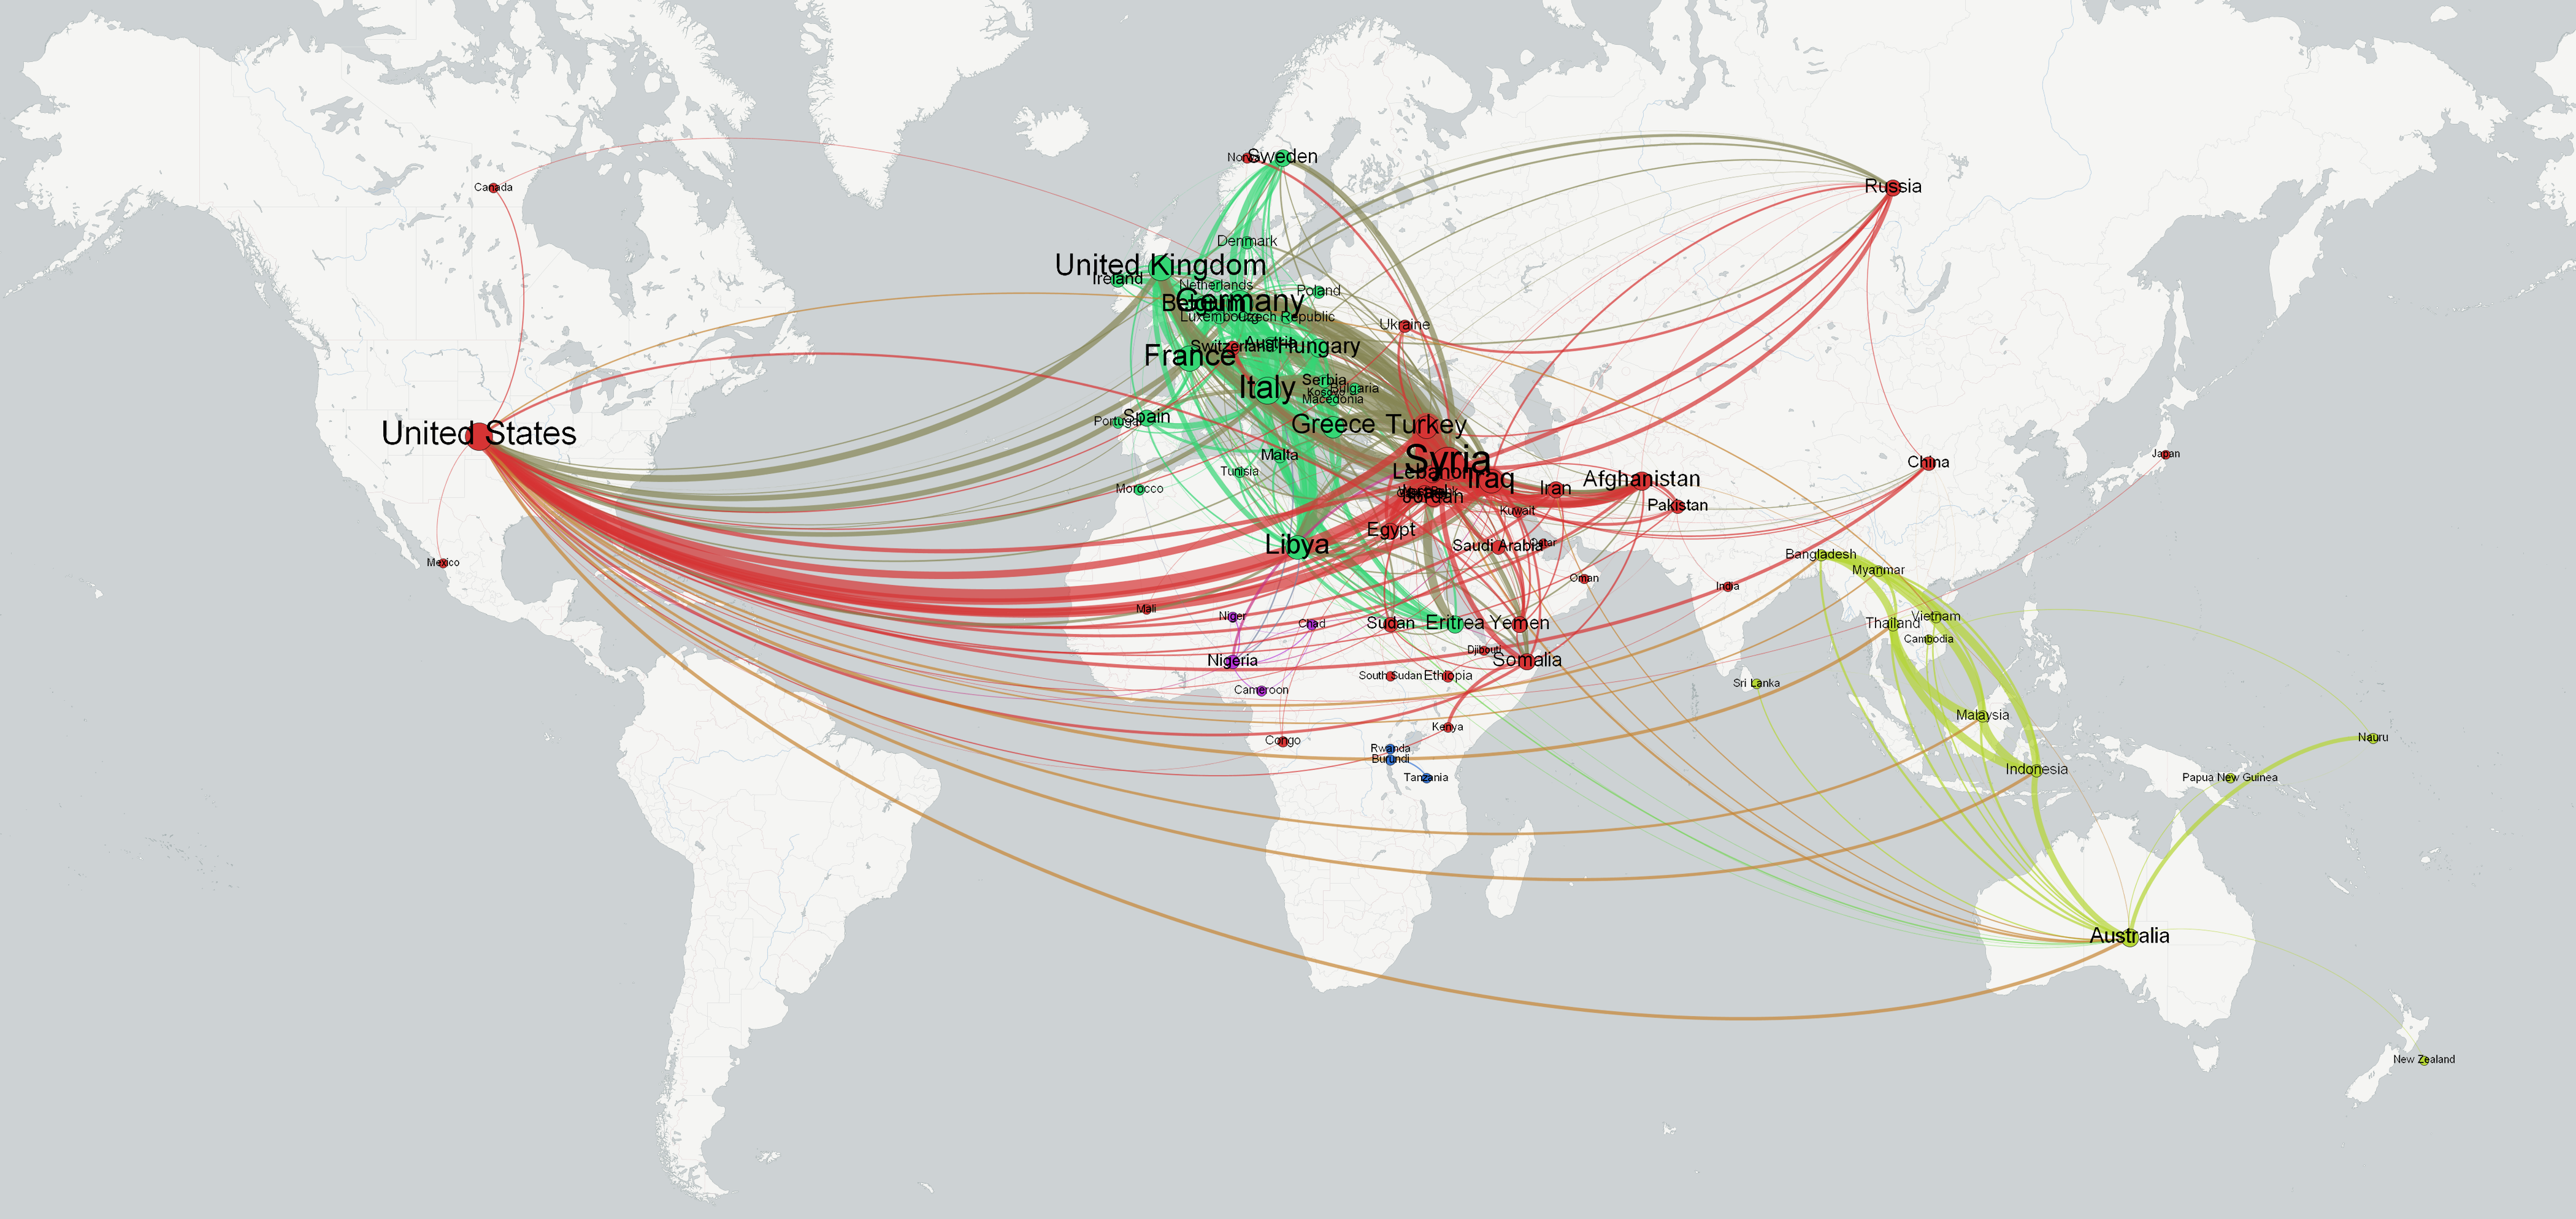
\includegraphics[width=\linewidth]{images/global-refugee-network-geo}
		\caption{Global refugee network map}
	\end{center}
\end{figure}

\newpage
\section{Civil wars}

\subsection{Iran - PJAK conflict}
The Iran-PJAK (Kurdistan Free Life Party) conflict is an armed conflict between the Islamic Republic or Iran and the ethnic secessionist Kurdisch guerrilla group PJAK, which began back in 2004. The group had been carrying out attacks in the Kurdistan Province of Iran and other Kurdish-inhabited areas. Following large clashes in summer 2011, a cease-fire was declared between the parties, with Iran claiming victory and PJAK ending all armed operations as of 29 September 2011. Since then, several violent incidents have occurred.

\begin{itemize}
	\item \textbf{Iran}
		\subitem supported by \textbf{Turkey}
	\item \textbf{Kurdistan Free Life Party (PJAK)}
\end{itemize}

Since the Iranian Revolution, there has been an ongoing conflict between Iran’s central government and Kurdish political movements rooted in the predominantly Kurdish region of western Iran. The level of violence has ebbed and flowed with peaks of serious conflict in 1979, the early eighties and the early nineties.

Kurdish casualties are estimated by the Kurdish Democratic Party of Iran (KDPI) at more than 30,000 civilian dead in addition to 4,000 Kurdish fighters. Along with the dead, there have been tens of thousands of people imprisoned, hundreds of villages destroyed and hundreds of thousands of people displaced. The local economy of an already under-developed region has been severely damaged by the conflict, as of course has the Iranian economy as a whole.

According to founding members of PJAK, however, the group began in Iran around 1997 as an entirely peaceful student-based human rights movement. The group was inspired by the success of Iraq's Kurdish autonomous region. Discouraged by the failure of previous Kurdish revolts, however, PJAK's leaders initially worked only to maintain and build a Kurdish national identity and to thwart the Iranian government's attempts to re-brand Iranian Kurds as ethnic Persians or Aryans.
PJAK transformed from a civil rights movement to a more ambitious and multi-directional independence movement.
\newpage



\begin{figure}[!h]
	\begin{center}
		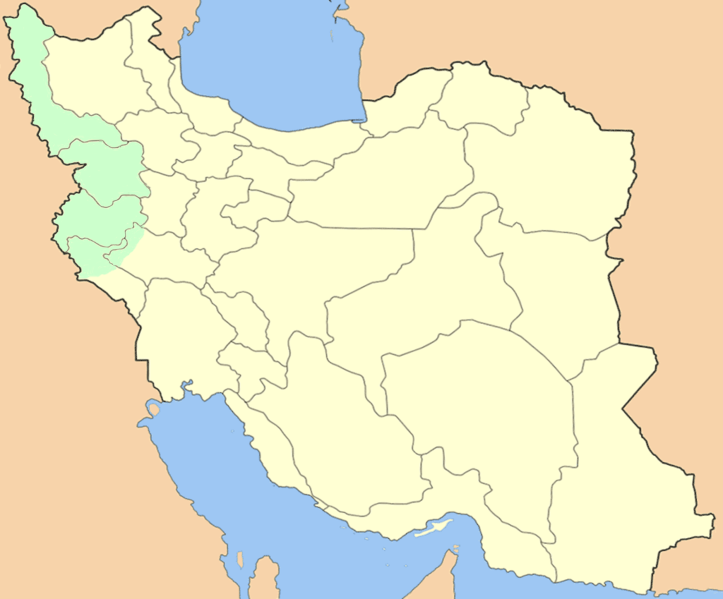
\includegraphics[width=0.5\linewidth]{images/Map_of_Iranian_Kurdistan}
		\caption{Map of Iranian Kurdistan}
	\end{center}
\end{figure}

It is clear to see the green marked area on the map, this is the epicenter of PJAK insurrection.
Following regions are included:
\begin{itemize}
	\item West-Azerbaijan
	\item Kordestan
	\item Kermanshah Provinces in Iran
	\item Kurdistan Region
\end{itemize}

There are not many reports or data to rely on, because every party involved in this civil war, accused others instead of taking fault on themselve. \textbf{So summed up following facts clearly point out:}

\begin{itemize}
	\item Iran vs Kurdistan Free Party (PJAK)
	\item around 34,000 casualties
	\item PJAK build on a national identity
	\item War Zone - West area of Iran
	\item Facts are not proven completely
\end{itemize}

\subsection{Syria Civil War}
Syria has been going through a brutal civil war for four years now. In 2011, Syria many government protests broke out.
Back then the current president with the name ''Bashar al-Assad'' did not appreciate these and responded with a massive killing spree, killing those who disagreed with him. This prompted resistors to build groups, and arm them with lethal weapons against him. This developed into a full-blown civil war, with at least a thousand of rebel groups with different mindsets.

Both sides leaked information, about having chemical weapons in their property. In August 2013, images surfaced that appeared to show a massive chemical attack on civilians in Syria. The United States blamed Assad and Assad blamed the rebels.
For a time it looked like the US was on the brink of military intervention in Syria. Then the UN (United Nations) and Assad cut a deal, to destroy all chemical weapons. The talk of intervention cooled off, for a while. \newline


\textbf{Main belligerents: }
\begin{itemize}
	\item \textbf{Syrian Goverment (NPF)}
		\subitem supported by Russia
	\item \textbf{Opposition}
		\subitem supported by United States
	\item \textbf{ISIL (ISIS)}
	\item \textbf{Army of Conquest}
	\item \textbf{Rojava (SDC)}
	\item \textbf{Combined Joint Task Force}
		\subitem US, States of Europe, Turkey, Saudi Arabia
\end{itemize}

\newpage

\begin{figure}[!h]
	\begin{center}
		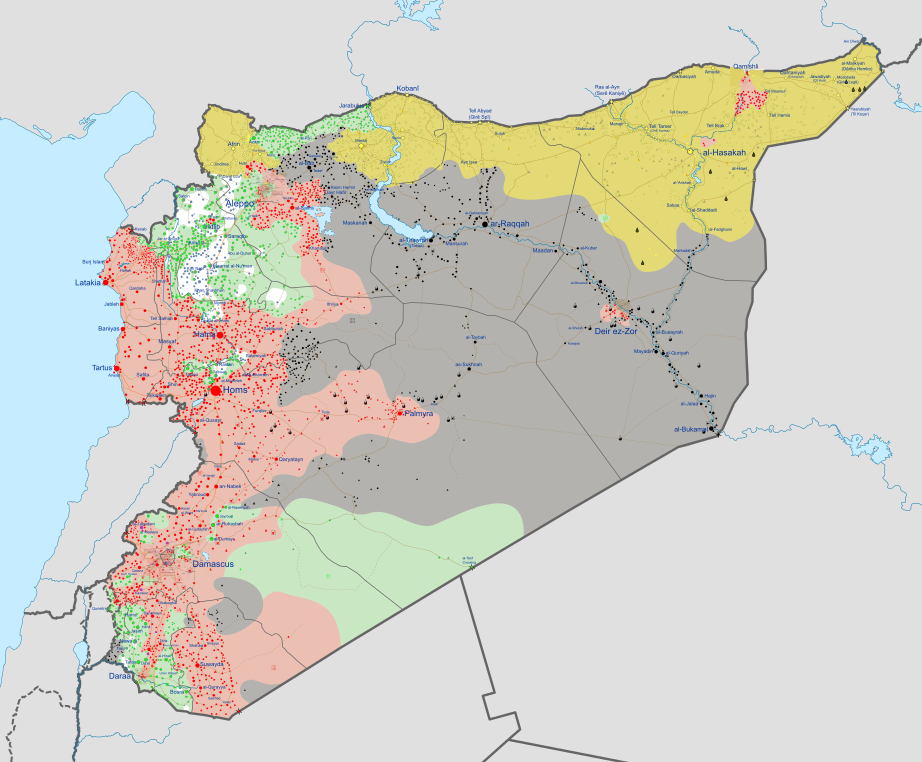
\includegraphics[width=\linewidth]{images/Syrian_Civil_War_map}
		\caption{Syrian civil war map}
	\end{center}
\end{figure}

\textbf{current military situation:}\newline
\textit{Red}: \textbf{Syrian Goverment}
\textit{Green}: \textbf{Syrian Oppostition}
\textit{Yellow}: \textbf{Federation of North Syria (SDF)}
\textit{Grey}: \textbf{Islamic State of Iraq and the Levant}
\textit{White}: \textbf{Jabhat Fateh al-Sham}

\newpage

At the start of the war, discontent against the government was said to be the strongest in Syria's poor areas, predominantly among conservative Sunnis. These included cities with high poverty rates, such as Daraa and Homs and the poorer districts of large cities.

Socioeconomic inequality increased significantly after free market policies were initiated by Hafez al-Assad in his later years, and accelerated after Bashar al-Assad came to power. With an emphasis on the service sector, these policies benefited a minority of the nation's population, mostly people who had connections with the government, and members of the Sunni merchant class of Damascus and Aleppo. The country also faced particularly high youth unemployment rates.

This coincided with the most intense drought ever recorded in Syria. It lasted from 2007 to 2010 and resulted in widespread crop failure, an increase in food prices and a mass migration of farming families to urban centers. Syria had also received in the same period around 1.5 million refugees from Iraq.

By 2011, Syria was facing steep rises in the prices of commodities and a clear deterioration in the national standard of living.

\textbf{So summed up following facts clearly point out:}
\begin{itemize}
	\item Al-Assad vs. Rebels vs. World
	\item origin of modern refugee crisis
	\item chemical weapons
	\item thousands of rebel-groups with different mindsets
	\item human rights
\end{itemize}



\subsection{USA vs. Russia, War for resources}
The Syrian war often seems like a big confusing mess but one factor that is not often mentioned could be the key to unlocking the conflict.
Many have questioned why Russia became involved in the Syrian war but often overlook the fight over natural gas.
Russia currently supplies Europe with a quarter of the gas it uses for heating, cooking, fuel and other activities.
In fact 80 per cent of the gas that Russian state-controlled company Gazprom produces is sold to Europe, so maintaining this crucial market is very important.
But Europe does not like being so reliant on Russia for fuel and has been trying to reduce its dependence. It’s a move that is supported by the United States as it would weaken Russian influence over Europe.
This has not gone down well with Russia, which uses its power over gas as political leverage and has a history of cutting off supply to countries during conflicts. It has even gone to war in Georgia and Ukraine to disrupt plans to export gas from other parts of the Middle East.
Russia has always used gas as an instrument of influence. The more you owe Gazprom, the more they think they can turn the screws.Much of Russia’s power comes from established pipelines used to transport gas to Europe cheaply. But other countries are now trying to get around Russia and provide new sources of gas to Europe.
In 2015 US President Barack Obama spoke openly about the need for Europe to reduce its reliance on Russian gas following the conflict in Ukraine.
The US also wants to use its own natural gas supply, recently developed through fracking, to undercut Russian supply. But it will be years before the US will be in a position to ship this overseas.
The US is not the only country trying to outmanoeuvre Russia, and this is where the role of Syria becomes more important.

\textbf{Two new pipelines} \newline
Before the civil war, two competing pipelines put forward by Qatar and Iran aimed to transport gas to Europe through Syria.
Qatar’s plans were first put forward in 2009 and involved building a pipeline from the Persian Gulf via Saudi Arabia, Jordan, Syria and Turkey.
The gas field located 3000 metres below the floor of the Persian Gulf is the largest natural gas field in the world. Qatar owns about two-thirds of the resource but can’t capitalise on it fully because it relies on tankers to deliver it to other countries and this makes its gas more expensive than Russia’s.
It was hoped the pipeline would provide cheaper access to Europe but Syrian President Bashar al Assad refused to give permission for the pipeline to go through his territory. Some believe Russia pressured him to reject the pipeline to safeguard its own business.


\begin{figure}[!h]
	\begin{center}
		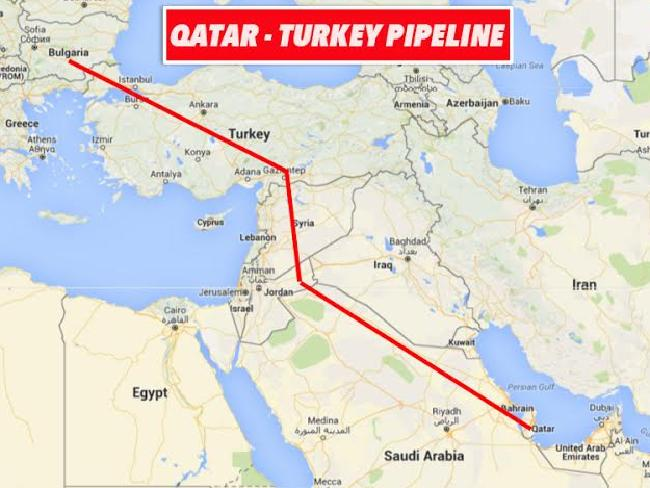
\includegraphics[width=0.5\linewidth]{images/pipe_line_turkey}
		\caption{The proposed gas pipeline from Qatar via Saudi Arabia, Jordan, Syria and Turkey to Europe.}
	\end{center}
\end{figure}

\newpage
In the meantime Iran, which owns the other smaller, share of the Persian Gulf gas field, decided to lodge its own rival plan for a \$10 billion pipeline to Europe via Iraq and Syria and then under the Mediterranean Sea.

\begin{figure}[!h]
	\begin{center}
		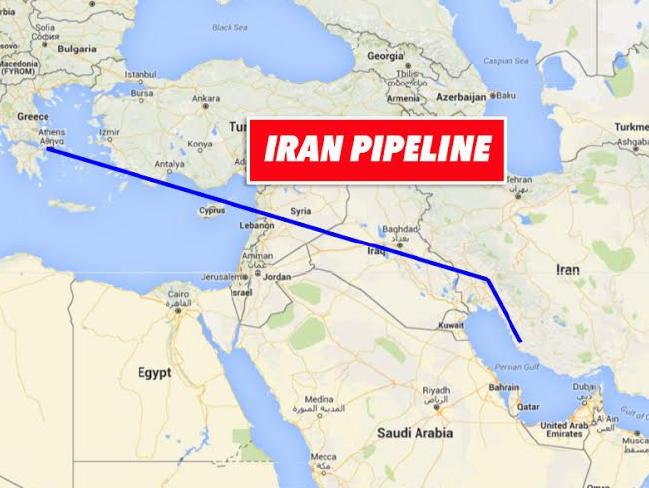
\includegraphics[width=0.5\linewidth]{images/pipe_line_iran}
		\caption{Pipeline from Iran via Iraq and Syria to Europe.}
	\end{center}
\end{figure}

These plans apparently had Russia’s blessing, possibly because it could exert more influence over Iran, which, unlike Qatar, did not host a US air base.
Assad signed off on the Iran plan in 2012 and it was due to be completed in 2016 but it was ultimately delayed because of the Arab Spring and the civil war.
Many countries supporting or opposing the war against Assad have links to these pipeline plans.
Failed pipeline bidder Qatar is believed to have funded anti-Assad rebel groups by \$3 billion between 2011 and 2013. Saudi Arabia has also been accused of funding the terrorist group.
In contrast Orenstein and Romer noted the successful pipeline bidder, Iran, was believed to be helping Assad by running the Syrian army, supplying it with weapons and even troops.

Viewed through a geopolitical and economic lens, the conflict in Syria is not a civil war, but the result of larger international players positioning themselves on the geopolitical chessboard in preparation for the opening of the pipeline.
Just as the 2003 Iraq War has been linked to oil in the Persian Gulf, Syria may turn out to be all about gas.


\subsection{ISIS}
Civil wars are not the only reason for this crisis. Weak economies causing the population to leave their places and find better ones, with more stable political and social environment. And if that is not enough, an organisation called ISIS (Islamic State of Iraq and Syria) developed through this time. They use the downsides of these developing countries for their advantage. Recruiting young people to fight on their side for their ideology.

\section{The civil war in Syria}

Syria has been going through a brutal civil war for four years now. In 2011, Syria many government protests broke out.
Back then the current president with the name ''Bashar al-Assad'' did not appreciate these and responded with a massive killing spree, killing those who disagreed with him. This prompted resistors to build groups, and arm them with lethal weapons against him. This developed into a full-blown civil war, with at least a thousand of rebel groups with different mindsets.

Both sides leaked information, about having chemical weapons in their property. In August 2013, images surfaced that appeared to show a massive chemical attack on civilians in Syria. The United States blamed Assad and Assad blamed the rebels.
For a time it looked like the US was on the brink of military intervention in Syria. Then the UN (United Nations) and Assad cut a deal, to destroy all chemical weapons. The talk of intervention cooled off, for a while.

One of the most famous rebel group named ISIS has been indirectly helpful to Assad, since he has been more focused on defeating other organisations, that set their goal to take him down, ISIS was fighting other rebel groups instead of him.
This renderd ISIS the opportunity to take more land under their control and become even more powerful. So powerful that last September, the US started for the first time with airstrikes.

\section{How are they getting to the EU?}
Most of the people are paying smugglers for spots on overcrowded fishing boats or inflatable dinghies (little boats), trains or buses. Thousands of them have died while trying to make it to the EU.

One big disaster happended on the 26th of August 2015. 71 refugees died inside a reefer, which was on the way from Hungary towards Austria. It was found next to a village called ''Pandorf'' on a highway without a driver. As the police arrived, decay liquid was already dropping out of the truck. The responsible organization for this disaster is a hungarian smuggler group.

\section{EU on the edge of its breakdown}
Allthough Germany has had the most asylum applications in 2015, Hungary had the highest in proportion to its population, despite having closed its border with Croatia in an attempt to stop the flow in October. Nearly 1,800 refugees per 100,000 of Hungary´s local population claimed asylum in 2015.

Sweden followed close behind with 1,667 per 100,000.

The figure for Germany was 587 and for the UK it was 60 applications for every 100,000 residents. The EU average was 260.

\begin{figure}[!h]
	\begin{center}
		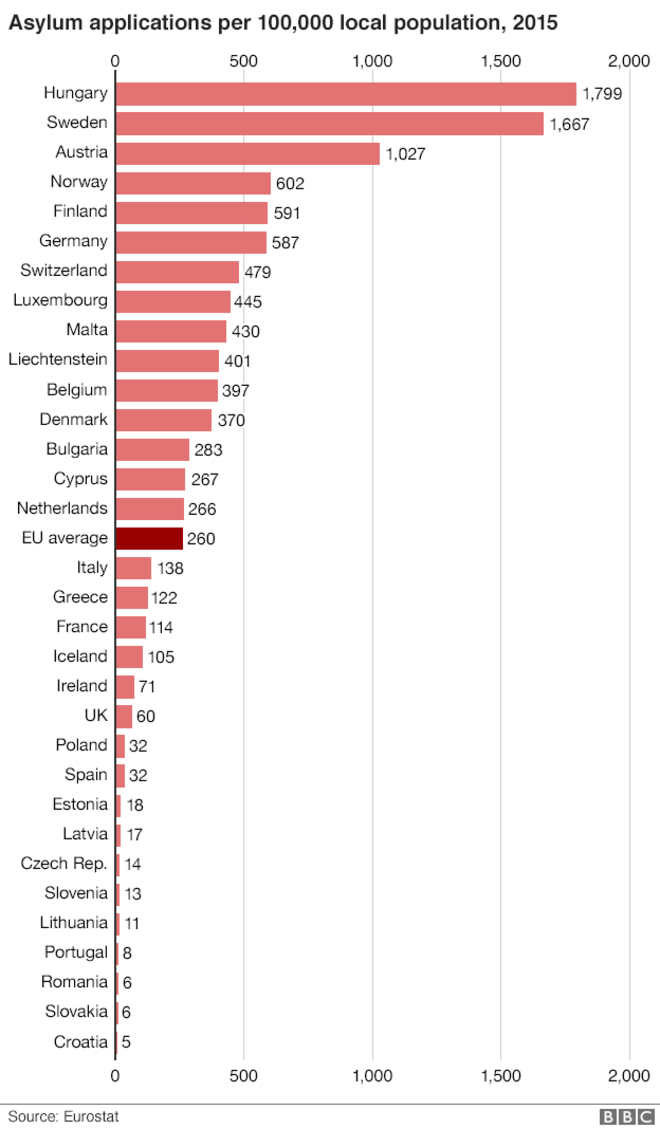
\includegraphics[width=0.5\linewidth]{images/asylums_per_100k}
		\caption{Asylum applications per 100,000 local population}
		\label{broker}
	\end{center}
\end{figure}

\subsection{Response from Europe}
The European Union decided to evenly redistribute about 160,000 refugees EU-wide particulary from countries where the majority of migrants have been arriving. Affected countries are Italy, Greece. The following chart will describe the relocation-plan of the Union.

\begin{figure}[!h]
	\begin{center}
		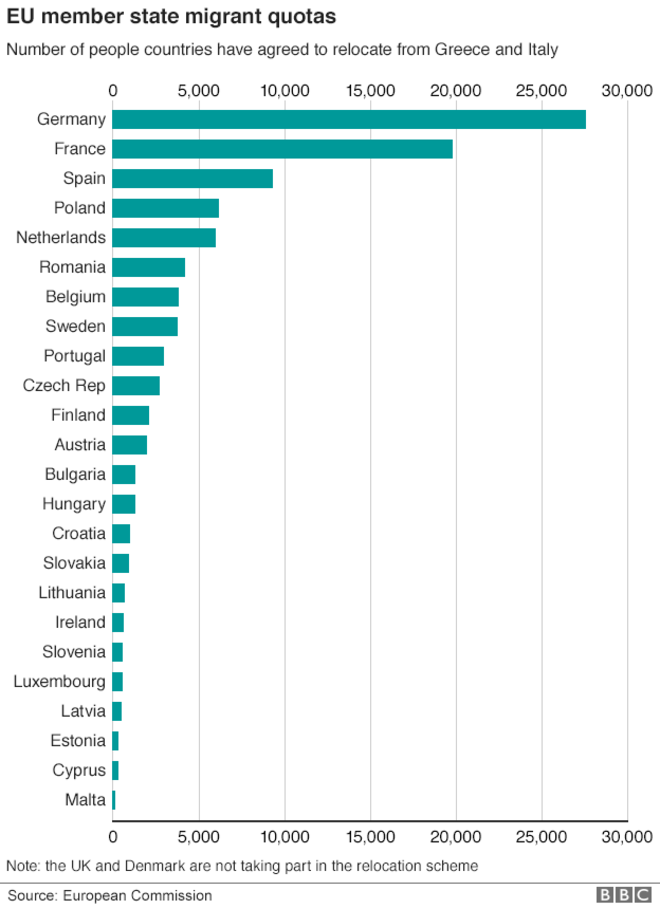
\includegraphics[width=0.5\linewidth]{images/asylums_redistribution}
		\caption{Number of people countries have agreed to relocate from Greece and Italy}
		\label{broker}
	\end{center}
\end{figure}
\newpage
\section{Has the refugee crisis uncovered the downsides of \mbox{globalization}?}

According to information gathered in 2013, there are 232 million of migrants. Migrant waves are mostly heading towards USA, Russia and Europe. These are mainly economic migrants. Others are forced migrants or refugees affected by wars or deconstruction of countries due to export of democracy and search for vast oil fields in the Middle East and all over the world. Refugee crisis in Europe encompasses economic, forced, illegal migrants and refugees. It is a heterogenous group on the move or a new Migration Period in the age of the second modernity. They are being currently used as a powerful biopolitical and potential economic weapon in conquering space and transforming cultural identities in the long run, as it is the case in Europe. Europe is being confronted with an unexpected refugee crisis. The case of refugee crisis, which exemplifies and shows the ugly side of globalization, has made Europe look like a bad tempered instrument of imaginary power in evident postmodern condition.

Multinational corporations are accused of social injustice, unfair working conditions, as well as lack of concern for environment, mismanagement of natural resources, and ecological damage. This causes many people to leave and find better places to live, like mentioned before.

\section{Conclusion}
Refugees have been accepted

